\documentclass[runningheads]{llncs}
\usepackage{graphicx}
\usepackage{booktabs}
\usepackage{amsmath,amssymb}
\usepackage{url}
\usepackage{multirow}

\graphicspath{{figures/}}
\urlstyle{same}
\pagestyle{headings}
\titlerunning{Hardware-Calibrated Progressive Temporal Reuse}
\authorrunning{Anonymous Submission}

\begin{document}

\title{Hardware-Calibrated Progressive Temporal Reuse for Efficient Video Semantic Segmentation}
\author{Anonymous Submission}
\institute{Anonymous for Double-Blind Review}

\maketitle

\begin{abstract}
Temporal reuse can reduce redundant video segmentation work, but a fixed reuse policy does not account for frame-wise drift or target-device stage costs. We present Hardware-Calibrated Progressive Reuse (HCPR), a lightweight controller for SegFormer that progressively chooses among whole-stage reuse boundaries using normalized temporal drift and measured marginal stage costs. HCPR keeps the segmentation model, decoder, precision, and data protocol fixed while changing only the cached suffix reused on each frame. On VSPW, the same frozen temporal calibration transfers from an RTX 4090 D to an RTX 3080 Ti after target-device stage profiling, without retraining or $\lambda$ recalibration. At the lowest-damage tested point, HCPR reaches 1.354$\times$ speedup with a 0.0726 percentage-point mIoU drop for B0 and 1.344$\times$ with a 0.1193-point drop for B1. Physical stage-call counters verify real compute omission, and controller overhead is included in paired end-to-end CUDA latency.
\keywords{Hardware-aware inference \and SegFormer \and Temporal feature reuse \and Video semantic segmentation \and VSPW}
\end{abstract}

\section{Introduction}
Video semantic segmentation repeatedly applies an image model to temporally redundant frames. Keyframe propagation and multi-rate execution exploit this redundancy \cite{zhu2017dff,shelhamer2016clockwork,jain2019accel}, but a practical streaming system must answer two coupled questions: how much of a hierarchical model can be reused on the current frame, and which continuation is worthwhile on the target GPU? A fixed interval or fixed boundary cannot jointly express temporal change and unequal stage cost.

Temporal Feature Correlation (TFC) is particularly close to this problem. TFC uses low-level cosine similarity to guide feature interpolation and sparse multi-scale deformable attention, reporting both semantic accuracy and mean Video Consistency (mVC) on VSPW \cite{lin2024tfc}. We add its published numbers as a quantitative positioning reference in Table~\ref{tab:tfc}, while keeping the protocol boundary explicit: TFC uses a learned interpolation/MSDA model, 480$\times$853 inference, a four-frame keyframe interval, and GTX 1080 timing, whereas HCPR uses a frozen SegFormer checkpoint, 512$\times$512 inference, whole-stage reuse, and paired CUDA timing on two different GPUs. These values are therefore not an apples-to-apples head-to-head comparison; they prevent the nearest prior work from being left without numerical context.

We make the boundary question explicit using SegFormer \cite{xie2021segformer}. The paper does not propose a new backbone or a TFC replacement. Instead, it defines three auditable whole-stage reuse boundaries, keeps the decoder and required fresh prefix unchanged, and evaluates their interaction with fixed intervals and progressive routing on SegFormer-B0 and B1.

Our contributions are threefold:
\begin{itemize}
\item We formulate progressive whole-stage reuse over four actions: S2--S4, S3--S4, S4, and Full, using per-boundary drift and a bounded stale-age guard.
\item We normalize continuation scores by measured target-device marginal stage cost, enabling profile-only transfer of frozen temporal scales and thresholds across two evaluated GPU generations.
\item We evaluate HCPR on VSPW with SegFormer-B0/B1 using paired CUDA latency, physical stage-call counters, and fixed-policy references. NewCost, OldCost, and DriftOnly ablations are also included.
\end{itemize}

\section{Related Work}
\textbf{Temporal feature reuse.} Deep Feature Flow propagates keyframe features with motion information, Clockwork Convnets assign different execution rates to network components, and Accel combines efficient segmentation with corrective fusion \cite{zhu2017dff,shelhamer2016clockwork,jain2019accel}. These works establish the value of temporal redundancy, while HCPR focuses on auditable selection among multiple hierarchical whole-stage suffixes.

\textbf{Efficient video segmentation.} Video methods have explored budget-aware frame selection, temporally consistent propagation, dynamic token processing, resolution changes for compressed video, and temporal adaptation \cite{baghbaderani2024bofp,liu2024dovit,hu2023arseg,zhang2022auxadapt}. TFC is the closest reported VSPW reference because it combines efficiency and stability; its external mVC and FPS values are listed separately in Table~\ref{tab:tfc}. HCPR has a different unit of reuse and does not add alignment, fusion, or sparse attention.

\textbf{Efficient segmentation Transformers.} SegFormer uses a hierarchical Mix Transformer encoder and lightweight multi-scale decoder \cite{xie2021segformer}; VSPW supplies the densely annotated video benchmark \cite{miao2021vspw}. RTFormer represents a complementary direction that designs a real-time Transformer segmentation model directly \cite{wang2022rtformer}. Our focus is runtime reuse inside a frozen model and the relationship between temporal drift, skipped computation, and target-device stage economics.

\begin{table}[t]
\centering
\caption{Published quantitative TFC positioning on VSPW, transcribed from \cite{lin2024tfc}. These rows are external references, not matched HCPR measurements. mVC8/mVC16 are mean Video Consistency at the corresponding clip lengths.}
\label{tab:tfc}
\small
\setlength{\tabcolsep}{3.5pt}
\begin{tabular}{lccccc}
\toprule
Method & Backbone & mIoU & mVC8 & mVC16 & FPS \\
\midrule
SegFormer + TFC & MiT-B0 & 32.9 & 85.3 & 80.0 & 38.2 \\
SegFormer + TFC & MiT-B1 & 36.7 & 86.8 & 81.5 & 37.1 \\
\bottomrule
\end{tabular}
\end{table}

\section{Hardware-Calibrated Progressive Reuse}
\subsection{Whole-stage execution contract and cache semantics}
Let $F_i(t)$ denote the output of encoder stage $i$ for frame $t$. The frozen SegFormer path is
\begin{equation}
F_1(t) \rightarrow F_2(t) \rightarrow F_3(t) \rightarrow F_4(t) \rightarrow D(t),
\end{equation}
where $D$ is the decoder. HCPR always computes $F_1$ and $D$. On a reuse frame it may stop after a fresh prefix and reuse a cached suffix:
\begin{align}
\mathrm{S2\text{-}S4}:&\quad D(F_1(t),\widehat F_2,\widehat F_3,\widehat F_4),\\
\mathrm{S3\text{-}S4}:&\quad D(F_1(t),F_2(t),\widehat F_3,\widehat F_4),\\
\mathrm{S4}:&\quad D(F_1(t),F_2(t),F_3(t),\widehat F_4).
\end{align}
A Full action computes all stages and updates all cache entries. A hat denotes a cached final stage output, not an estimate of the current feature. Cache state resets at video boundaries and the first frame is Full. A stopped suffix is absent from the forward path rather than computed and masked.

\begin{figure}[t]
\centering
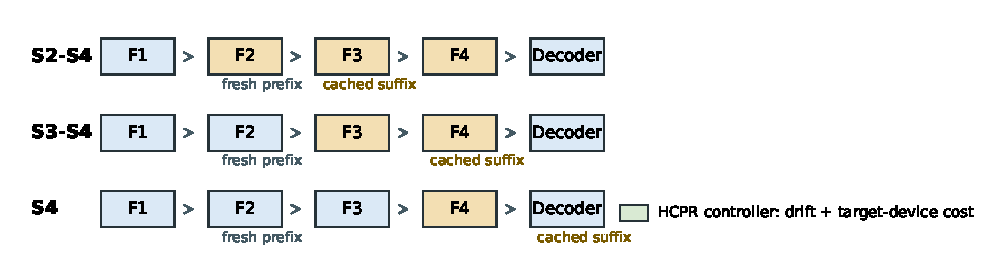
\includegraphics[width=.92\textwidth]{hcpr_method.pdf}
\caption{HCPR selects a progressive whole-stage route. The fresh prefix and cached suffix change by action, while the decoder remains active on every frame.}
\label{fig:method}
\end{figure}

HCPR maintains cache entries $C_2,C_3,C_4$ and pooled references at the three successive boundaries. When stage $i+1$ is recomputed, its upstream reference is refreshed from the current $F_i(t)$. References can therefore have different ages under dynamic routing. A separate age counter is tracked for each stage, and an age guard forces Full refresh after at most seven consecutive stale frames. Skipping Stage 2 necessarily skips every deeper stage, and skipping Stage 3 necessarily skips Stage 4.

\subsection{Progressive decision, drift, and hardware cost}
Stage 1 is first computed for every frame and compared with the reference associated with Stage 2. If HCPR stops there, Stages 2--4 are skipped. If it continues, Stage 2 is executed and a second test decides whether Stages 3--4 are recomputed; continuing again reaches the Stage-4 decision. Thus Full is the result of three successive continue decisions, not a separate frame classifier.

For boundary $i\in\{1,2,3\}$, the FP32 temporal drift is
\begin{equation}
d_i(t)=1-\cos(\operatorname{GAP}(F_i(t)),R_{i\rightarrow i+1}),\qquad
z_i(t)=\frac{d_i(t)}{s_i+\epsilon},
\end{equation}
where $s_i$ is the p90 drift estimated from 32 training videos. Segmentation labels do not enter the computation of $s_i$, $\lambda$, or any routing decision.

Let $c_j^{(h)}$ be the measured marginal cost of downstream stage $j$ on hardware $h$, and let $T_{\mathrm{full}}^{(h)}$ be the measured full-model profile. We define
\begin{equation}
k_j^{(h)}=\frac{c_j^{(h)}}{T_{\mathrm{full}}^{(h)}},\qquad
q_i(t,h)=\frac{z_i(t)}{k_{i+1}^{(h)}}.
\end{equation}
HCPR continues through boundary $i$ when $q_i(t,h)>\lambda$; otherwise it stops and reuses the remaining suffix. This is an empirically evaluated routing rule, not a claim of theoretical optimality.

We use seven pre-specified operating points, from Q20 through Q95, spanning conservative to aggressive reuse. The grid is derived from unlabeled calibration-score statistics and is not selected by validation mIoU. When the target GPU changes, only $c_2,c_3,c_4$ and $T_{\mathrm{full}}$ are remeasured; the model and controller parameters remain frozen.

\section{Experimental Protocol}
\paragraph{Dataset and models.} We use the official VSPW validation split: 343 videos, 24,392 RGB/ground-truth pairs, 124 classes, and ignore label 255 \cite{miao2021vspw}. We evaluate frozen VSPW-compatible SegFormer-B0 and B1 checkpoints at $512\times512$, batch size one, with BF16 autocast. No model, split, resolution, decoder, or training procedure changes between devices.

\paragraph{Calibration and temporal consistency metric.} Temporal scales and the seven operating-point thresholds are derived from 32 VSPW training videos with seed 42 and labels unused. For context, we use the mVC definition from TFC: for a video clip, it measures the agreement between the common ground-truth area and the common predicted area across frames \cite{lin2024tfc}. The archived HCPR Round 11 outputs contain aggregate mIoU, route, latency, and stage-call records but not the per-frame predicted masks required to recompute mVC8/mVC16 under that definition. We therefore do not fabricate an HCPR mVC number; Table~\ref{tab:tfc} reports the closest published quantitative reference, and the absence of a matched HCPR mVC comparison is an explicit limitation.

\paragraph{Hardware and timing.} The source device is an NVIDIA GeForce RTX 4090 D and the target device is an NVIDIA GeForce RTX 3080 Ti. Both runs use CUDA 11.8, PyTorch 2.1.2+cu118, and Transformers 4.44.2; the NVIDIA driver differs. We therefore describe the result as cross-device validation under matched framework/runtime versions rather than pure hardware isolation. Formal latency starts from a CUDA-resident model input and ends at ready segmentation logits. It includes HCPR pooling, cosine drift, normalization, scalar synchronization, Python branching, cache bookkeeping, selected fresh stages, and decoder. Video decoding, disk I/O, pageable host-to-device transfer, visualization, and result writing are excluded. Each configuration uses 200 warmup iterations, 1,000 CUDA-event measurements, five repetitions, and an immediately paired Full baseline in the same process.

\section{Results}
\subsection{Quality--latency operating points}
Table~\ref{tab:cross} reports representative HCPR-NewCost anchors. Full mIoU is 30.129 for B0 and 37.160 for B1; each drop is relative to its full model. At the lowest-damage target-device points, HCPR reaches 1.354$\times$/0.0726 pp for B0 and 1.344$\times$/0.1193 pp for B1. At $Q95$, B0 reaches 2.010$\times$/1.394 pp and B1 reaches 2.093$\times$/2.179 pp.

\begin{table}[t]
\centering
\caption{HCPR-NewCost cross-device results. Each cell reports paired end-to-end speedup / mIoU drop in percentage points. Full mIoU is 30.129 for B0 and 37.160 for B1.}
\label{tab:cross}
\small
\setlength{\tabcolsep}{4pt}
\begin{tabular}{llccc}
\toprule
Model & Device & Q20 & Q65 & Q95 \\
\midrule
B0 & RTX 4090 D & 1.229 / 0.073 & 1.657 / 0.442 & 1.836 / 1.379 \\
B0 & RTX 3080 Ti & 1.354 / 0.073 & 1.838 / 0.428 & 2.010 / 1.394 \\
B1 & RTX 4090 D & 1.323 / 0.115 & 1.707 / 0.830 & 1.919 / 2.122 \\
B1 & RTX 3080 Ti & 1.344 / 0.119 & 1.849 / 0.875 & 2.093 / 2.179 \\
\bottomrule
\end{tabular}
\end{table}

\begin{figure}[t]
\centering
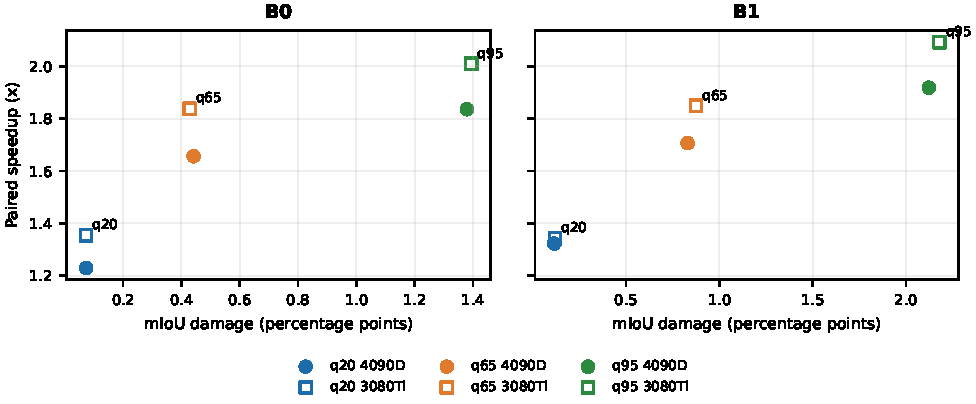
\includegraphics[width=.92\textwidth]{hcpr_cross_hardware_pareto.pdf}
\caption{Matched HCPR-NewCost anchors on the two evaluated GPUs. Filled circles denote RTX 4090 D and open squares denote RTX 3080 Ti.}
\label{fig:pareto}
\end{figure}

\subsection{Fixed-policy reference points}
For an internal non-dominance check, we remeasure five periodic whole-stage policies under the same paired timing contract. Table~\ref{tab:fixed} lists every value rather than only asserting a frontier. The same five points are used for both model scales: S4/FI-2, S3--S4/FI-2, S2--S4/FI-2, S2--S4/FI-4, and S2--S4/FI-8.

\begin{table}[t]
\centering
\caption{Complete five-point fixed-policy reference set. Speedup is paired end-to-end mean; quality is mIoU drop in percentage points.}
\label{tab:fixed}
\small
\setlength{\tabcolsep}{3.5pt}
\begin{tabular}{llrr|llrr}
\toprule
\multicolumn{4}{c|}{B0} & \multicolumn{4}{c}{B1} \\
Boundary & Interval & Drop & Speedup & Boundary & Interval & Drop & Speedup \\
\midrule
S4 & FI-2 & 0.091 & 1.068 & S4 & FI-2 & 0.118 & 1.111 \\
S3--S4 & FI-2 & 0.184 & 1.254 & S3--S4 & FI-2 & 0.283 & 1.331 \\
S2--S4 & FI-2 & 0.231 & 1.505 & S2--S4 & FI-2 & 0.397 & 1.554 \\
S2--S4 & FI-4 & 0.825 & 2.057 & S2--S4 & FI-4 & 1.280 & 1.952 \\
S2--S4 & FI-8 & 1.835 & 2.396 & S2--S4 & FI-8 & 2.715 & 2.282 \\
\bottomrule
\end{tabular}
\end{table}

The HCPR family supplies intermediate non-dominated operating points around this fixed reference set. On RTX 4090 D, all seven candidates are non-dominated against the five fixed-policy points for both B0 and B1. On RTX 3080 Ti, 7/7 B0 and 6/7 B1 candidates remain non-dominated. No HCPR point is claimed to strictly dominate the fixed frontier; the claim is a denser, drift-conditioned operating set.

\subsection{Complete source-device sweep and route allocation}
On RTX 4090 D, the seven-point HCPR sweep spans conservative to aggressive reuse. For B0, mIoU drop/speedup are 0.073/1.229, 0.190/1.478, 0.293/1.610, 0.442/1.657, 0.796/1.807, 0.988/1.785, and 1.379/1.836 at $Q20$ through $Q95$. For B1 they are 0.115/1.323, 0.282/1.605, 0.511/1.607, 0.830/1.707, 1.124/1.819, 1.690/1.837, and 2.122/1.919. The small B0 decrease from 1.807$\times$ at Q80 to 1.785$\times$ at Q90 has overlapping bootstrap confidence intervals and is treated as measurement noise, not as a meaningful violation of the overall trade-off.

Table~\ref{tab:routes} shows target-GPU route allocation. The dominant reuse action is S2--S4 because Stage 1 is always fresh; as the threshold becomes more permissive, Full execution falls from about 56\% at Q20 to about 15\% at Q95.

\begin{table}[t]
\centering
\caption{Target-GPU route allocation (\%). The operating-point header uses uppercase $Q$ to distinguish it from the framewise score $q_i$.}
\label{tab:routes}
\small
\setlength{\tabcolsep}{3.2pt}
\begin{tabular}{llrrrr}
\toprule
Model & Q & Full & S2--S4 & S3--S4 & S4 \\
\midrule
B0 & 20 & 56.50 & 42.22 & 1.24 & 0.05 \\
B0 & 65 & 26.50 & 70.31 & 2.94 & 0.26 \\
B0 & 95 & 15.27 & 81.67 & 2.54 & 0.53 \\
B1 & 20 & 56.00 & 43.83 & 0.13 & 0.04 \\
B1 & 65 & 26.61 & 72.27 & 0.97 & 0.14 \\
B1 & 95 & 15.21 & 82.81 & 1.48 & 0.49 \\
\bottomrule
\end{tabular}
\end{table}

Replacing the RTX 4090 D cost vector with the RTX 3080 Ti profile changes route allocation modestly for B0, with a maximum action shift of about 0.18 percentage points, and more visibly for B1. The largest B1 shift is a decrease of about 1.29 points in Full execution and an increase of about 1.34 points in S2--S4 at Q20. These are small changes in normalized-cost space, not a wholesale policy rewrite.

\subsection{Physical computation and stage economics}
At target-device Q20, Stage 1 and the decoder execute on all 24,392 frames, whereas Stage 4 executes 13,781 times for B0 and 13,659 times for B1. The corresponding F1/F2/F3/F4/D calls are (24,392, 14,094, 13,792, 13,781, 24,392) for B0 and (24,392, 13,700, 13,669, 13,659, 24,392) for B1. The counters are collected from forward modules rather than inferred from route labels.

The isolated controller costs 0.6431 ms for B0 and 0.6890 ms for B1 on RTX 3080 Ti, or 5.82\% and 6.25\% of the corresponding profiled Full times. The RTX 4090 D diagnostics are 0.7089 ms and 0.7548 ms. Formal speedup therefore already pays for pooling, cosine computation, normalization, scalar synchronization, branching, and cache bookkeeping.

\begin{table}[t]
\centering
\caption{Normalized stage-cost profiles used for target-device calibration.}
\label{tab:cost}
\small
\setlength{\tabcolsep}{4pt}
\begin{tabular}{llrrrr}
\toprule
Model & Device & $T_{\mathrm{full}}$ & $k_2$ & $k_3$ & $k_4$ \\
\midrule
B0 & RTX 4090 D & 7.793 & .234 & .243 & .197 \\
B0 & RTX 3080 Ti & 11.053 & .236 & .247 & .207 \\
B1 & RTX 4090 D & 7.563 & .236 & .240 & .195 \\
B1 & RTX 3080 Ti & 11.028 & .249 & .248 & .204 \\
\bottomrule
\end{tabular}
\end{table}

\subsection{Hardware-calibration ablation}
We compare HCPR-NewCost with HCPR-OldCost, which retains the RTX 4090 D cost vector on the target device, and ProgressiveDriftOnly, which sets all hardware costs to one. The complete anchor values are shown in Table~\ref{tab:ablation}. NewCost is strictly better on both axes than OldCost at B0/Q65, and strictly better on both axes than ProgressiveDriftOnly at B1/Q95. However, this is not a pointwise guarantee: OldCost is strictly better than NewCost on both axes at B1/Q20 and B1/Q65, two of the six model--anchor pairs.

The interpretation is therefore deliberately narrow. The normalized cost vectors of the two evaluated NVIDIA cards are very similar, so NewCost and OldCost differ mostly within the variation of the paired runs. The larger practical separation is between cost-aware routing and DriftOnly: at Q20, DriftOnly incurs roughly 5.7--6.0 times the NewCost quality damage; at Q65, the ratio is roughly 2.5--3.4 times. At Q95 the quality gap narrows, while DriftOnly may still trade quality for a different route distribution. Cost normalization matters as a transferable condition, but changing the vector between these two cards has only a small operating-point-dependent effect.

\begin{table}[t]
\centering
\caption{Target-device ablation at the three anchor operating points. Each entry is mIoU drop (pp) / paired speedup. Bold marks only the two strict NewCost improvements discussed in the text.}
\label{tab:ablation}
\small
\setlength{\tabcolsep}{2.5pt}
\begin{tabular}{llrrr}
\toprule
Model & Q & NewCost & OldCost & DriftOnly \\
\midrule
B0 & 20 & .073/1.354 & .073/1.356 & .414/1.679 \\
B0 & 65 & \textbf{.428/1.838} & .441/1.801 & 1.439/2.116 \\
B0 & 95 & 1.394/2.010 & 1.378/1.979 & 1.779/2.065 \\
B1 & 20 & .119/1.344 & \textbf{.115/1.379} & .711/1.849 \\
B1 & 65 & .875/1.849 & \textbf{.829/1.865} & 2.144/1.999 \\
B1 & 95 & \textbf{2.179/2.093} & 2.122/1.906 & 2.681/2.042 \\
\bottomrule
\end{tabular}
\end{table}

\subsection{Correctness and limitations}
The 100\% refresh equivalence gate passes for B0 and B1 at all three boundaries on 20 real validation frames, with maximum absolute error, mean absolute error, and relative L2 equal to zero. This verifies refresh and cache plumbing; it does not claim that a reused feature equals the current-frame feature. Physical counters provide the complementary compute proof that a stopped suffix is absent from the forward path.

The evidence covers one VSPW validation split, two SegFormer scales, two discrete NVIDIA desktop GPUs from different generations, one input resolution, and one matched framework/runtime family. The driver differs between hosts, so the study does not isolate hardware from every software-level effect. A new target GPU requires measuring its stage costs and rerunning the prescribed validation. Embedded SoCs, mobile GPUs, non-NVIDIA accelerators, custom kernels, and edge deployment remain untested. Most importantly for this revision, HCPR mVC8/mVC16 was not recomputed from archived per-frame masks under the TFC evaluation code; the external TFC numbers in Table~\ref{tab:tfc} must not be read as a direct HCPR comparison.

\section{Conclusion}
HCPR turns temporal reuse depth into a progressive per-frame decision conditioned on feature drift and measured downstream stage cost. On frozen VSPW SegFormer-B0 and B1 pipelines, it produces a dense speed--quality operating set and transfers from RTX 4090 D to RTX 3080 Ti using only a new stage-cost profile. The lowest-damage target-device points reach 1.354$\times$/0.0726 pp and 1.344$\times$/0.1193 pp speedup/drop for B0/B1, while more aggressive points exceed 2$\times$ speedup. The central claim is bounded: the study establishes physically verified whole-stage reuse and hardware-conditioned latency on the evaluated setup, while a matched HCPR temporal-consistency comparison remains future work.

\bibliographystyle{splncs04}
\bibliography{references}

\end{document}
